\documentclass[
% opciók nélkül: egyoldalas nyomtatás, elektronikus verzió
% twoside,     % kétoldalas nyomtatás
% tocnopagenum,% oldalszámozás a tartalomjegyzék után kezdődik
]{thesis-ekf}
\usepackage[T1]{fontenc}
\PassOptionsToPackage{defaults=hu-min}{magyar.ldf}
\usepackage[magyar]{babel}
\usepackage{mathtools,amssymb,amsthm,pdfpages}
\usepackage{enumitem, url}
\footnotestyle{rule=fourth}

\newtheorem{tetel}{Tétel}[chapter]
\theoremstyle{definition}
\newtheorem{definicio}[tetel]{Definíció}
\theoremstyle{remark}
\newtheorem{megjegyzes}[tetel]{Megjegyzés}

\begin{document}
	\institute{Matematikai és Informatikai Intézet}
	\title{A kommunikációs gráfok modelljeinek vizsgálata Python programozási nyelvvel}
	\author{Mohai Ferenc\\programtervező informatikus BSc}
	\supervisor{Dr.~Kusper Gábor\\egyetemi docens}
	\city{Eger}
	\date{2022}
	
	\maketitle
	\tableofcontents
	
	\chapter*{Bevezetés}
	\addcontentsline{toc}{chapter}{Bevezetés}
	A szakdolgozati szemináriumon, amikor hallottam Kusper Gábor tanár úr magyarázatát a kutatásról, annak eredményeiről, céljáról, felhasználásáról. és már akkor nagyon megtetszett a téma. A SAT megoldó széles körű felhasználásáról beszélgettünk. Korábbi előadásokon, gyakorlatokon is voltak tanáraim, akik ezt a témát felvetették, és már akkoriban meghozták a kedvemet hozzá. Amikor választanom kellett, nem volt nagy kérdés, hogy ez egy számomra érdekes téma, amivel szívesen dolgozok, és lehetőséget ad a fejlődésre.

	Szaktársammal, Rajna Franciskával csak mi ketten érdeklődtünk ebben a témában, úgyhogy mindenki örömmel beszélte meg a részleteket és közös megegyezéssel találtuk ki melyik ágát dolgozza ki a témának. Pozitív és energikus első benyomás után örömmel kezdtünk a munkának. Bíró Csaba és Balla Tamás tanár urakkal dolgoztunk a témával kapcsolatos házi TDK-hoz hasonló előadásokon és kutatásokon \cite{am} vettünk részt. Az egyik alkalommal egy plakátot is készítettünk, ezekkel megalapozva egy lendületes kezdést.
	
	Megbeszéltük hol szorul fejlesztésre a SAT megoldó, amin tudok programozással javítani. Valamint a korábbi általuk írt angol nyelvű szakirodalmakkal elsajátíthatom az elméleti hátteret, felzárkózhatok a jelenlegi helyzethez és ezeken dolgozva könnyedén belerázódjak a szakdolgozatom megfogalmazásába. Így kezdtem el a munkámat.
	
	\chapter{Az alapok}
	
	A munkámat azzal kezdtem, hogy szakirodalmakat olvastam, fordítottam és értelmeztem, amiket korábban témavezetőim írtak, ez \apageref{szakirodalom}.~oldalon olvasható. Anyagot gyűjtöttem és dolgoztam fel a SAT megoldókról. Ezekben megjelentek különböző definíciók, mint \aref{tautologia}.~definíció a tautológia, \aref{cnf}.~definíció a \textsc{cnf}, és \aref{dnf}.~definíció a \textsc{dnf}, valamint programozási nyelvek, mint a Python \aref{python-programnyelv}.~szakaszban és a Wolfram Alpha \aref{wolframalpha}.~szakaszban.
		
	\section{Szakirodalom}

	Alapfogalmak, definíciók:
	
	\begin{definicio}
		Atomi formula, röviden atom:  Azt mondjuk, hogy egy szimbólum atomi formula, vagy atom, akkor és csak akkor, ha egy kifejezést jelöl. Ilyen atomok, az igaz és hamis ítéletváltozók. Szimbólumuk általában az \emph{I} és \emph{H} betűk magyarul, de szoktuk használni az angol megfelelőjét is a \emph{T} és \emph{F} betűket.
	\end{definicio}

	\begin{definicio}
		Literál: Azt mondjuk, hogy egy szimbólum literál, akkor és csak akkor, ha egy atom, vagy annak negáltja.
	\end{definicio}

	\begin{definicio}		
		Jól formázott formula, röviden formula: Azt mondjuk, hogy egy szimbólum sorozat jól formázott formula, vagy formula, akkor és csak akkor, ha F formula a következő alakok egyikében van:
		\begin{enumerate}[label=\textit{(\alph*)}]
			\item A, ahol A egy atom;
			\item $ \neg A $, ahol A egy formula;
			\item $ (A \wedge B) $, ahol A és B formulák;
			\item $ (A \vee B) $, ahol A és B formulák;
			\item $ (A \implies B) $, ahol A és B formulák;
			\item $ (A \Leftrightarrow B) $, ahol A és B formulák.
		\end{enumerate}
		Minden formula a fenti esetek véges sokszori alkalmazásával áll elő.
	\end{definicio}

	\begin{definicio}
		Formula: Adott ítéletváltozónak egy véges, nem üres V halmaza.
		\begin{enumerate}
			\item Ítéletváltozó: ha $ A\in V $, akkor A formula.
			\item Negáció: ha A formula, akkor $\neg A $ is formula.
		\end{enumerate}
	\end{definicio}

	\begin{definicio}
		Operátor: Azt mondjuk, hogy egy szimbólum operátor, akkor és csak akkor, ha egy Formulán, klózon, vagy literálon módosítást végez, oly módon, hogy kiinduló állapotát megváltoztatja, megfelelő elő feltételek mellett. Azaz két ítéletváltozó értékéből, azokat értelmezve egy harmadik értéket eredményez.
	\end{definicio}
	
	\begin{definicio}
		Klóz, angolul clause: Azt mondjuk, hogy egy formula klóz, akkor és csak akkor, ha adott literáloknak és operátoroknak egy véges, nem üres, egynél több elemű W halmaza.

		Klózban értelmezve,
		\begin{enumerate}
			\item pozitív literál: ha $ B\in W $, és B egy pozitív literál.
			\item negatív literál: ha B pozitív literál, akkor $\neg B $ negatív literál.
			\item és operátor: ha $ B \wedge \neg B $, akkor $\wedge$ egy és operátor.
			\item vagy operátor: ha $ B \vee \neg B $, akkor $\vee$ egy vagy operátor.
		\end{enumerate}
		Pozitív vagy negatív literál is feltűnhet egy klózban, de sohasem egyszerre. Az is lehetséges, hogy valamelyik változó egyik formában sem tűnik fel egy klózban, hiszen egyszerűsíthetünk: $ B \wedge\neg B \equiv\emptyset $.
	\end{definicio}
	
	\begin{megjegyzes}
		Létezik konjunktív és diszjunktív klóz is. Vegyes egy klóz tartalma, ha vagy, valamint és operátorokat is tartalmaz.
	
		Diszjunktív klóz: Azt mondjuk, hogy $ l_{i} $ szimbólumok egy klózt alkotnak, akkor és csak akkor, ha minden $ l_{i} $ literál: $ l_{1}\vee\dots\vee l_{n} $
		
		Konjunktív klóz: Azt mondjuk, hogy $ l_{i} $ szimbólumok egy klózt alkotnak, akkor és csak akkor, ha minden $ l_{i} $ literál: $ l_{1}\wedge\dots\wedge l_{n} $
	\end{megjegyzes}

	\begin{definicio}
		Implikáció: Azt mondjuk hogy egy operátor implikáció, akkor és csak akkor, ha mindkét oldalán van egy literál, és egy harmadik literált állít elő a kettő értékéből, oly módon, hogy az összes bal oldali értékből pozitív literált állít elő, kivéve, ha a bal oldalán pozitív, a jobb oldalán negatív literál van.
		Mivel a negatív értékből nem következik a pozitív érték. Jelölése: $ A \implies B $
	\end{definicio}

	\begin{definicio}
		Ekvivalencia: Azt mondjuk, hogy egy operátor ekvivalencia, akkor és csak akkor, ha mindkét oldalán van egy literál, és egy harmadik literált állít elő a kettő értékéből, oly módon, hogy ha mindkét oldalán ugyan az a pólusú literál van, akkor pozitív literált állít elő, kivéve, ha eltérnek a pólusok. Jele: $ \equiv $
	\end{definicio}

	\begin{megjegyzes}
		Pólus alatt a negatív vagy pozitív jelzőt értjük.
	\end{megjegyzes}

	\begin{definicio}
		És operátor, más néven konjukció: Azt mondjuk, hogy egy operátor konjukció, akkor és csak akkor, ha mindkét oldalán van egy literál, és egy harmadik literált állít elő a kettő értékéből, oly módon, hogy ha mindkét oldalán pozitív literál van, akkor és csak akkor pozitív literált állít elő, különben negatív literált. Jele: $\wedge$
	\end{definicio}

	\begin{definicio}
		Vagy operátor, más néven diszjunkció: Azt mondjuk, hogy egy operátor diszjunkció, akkor és csak akkor, ha mindkét oldalán van egy literál, és egy harmadik literált állít elő a kettő értékéből, oly módon, hogy ha mindkét oldalán negatív literál van, akkor negatív literált állít elő, különben pozitív literált. Jele: $\vee$
	\end{definicio}

	\begin{definicio}\label{cnf} % megjegyzésbe kiemelni az angol megfelelőket? CNF DNF
		Konjunktív normál forma, röviden \textsc{knf}, angolul conjunctive normal form, röviden \textsc{cnf}: Azt mondjuk, hogy logikai formula konjunktív normál forma, akkor és csak akkor, ha egy vagy több klózt egymáshoz kötünk konjunkcióval.
	\end{definicio} % példákat cnfre, dnf-re

	\begin{definicio}\label{dnf}
		Diszjunktív normál forma, angolul disjunctive normal form, röviden \textsc{dnf}: Azt mondjuk, hogy logikai formula diszjunktív normál forma, akkor és csak akkor, ha egy vagy több klózt egymáshoz kötünk diszjunkcióval.
	\end{definicio}

	\begin{definicio}
		Interpretáció: Adott ítéletváltozóknak egy véges sok, nem üres V halmaza.
		Azt mondjuk, hogy a J hozzárendelés az F formula egy interpretációja, akkor és csak akkor, ha F minden atomjához vagy az igaz, vagy a hamis értéket rendeljük, de csak az egyiket.
	\end{definicio}

	\begin{definicio}\label{tautologia}
		Logikai törvény, más néven tautológia: Azt mondjuk, hogy az F formula logikai törvény, vagy tautológia, akkor és csak akkor, ha F minden interpretációjában igaz.
	\end{definicio}

	\begin{definicio}
		Logikai ellent mondás, angolul contradiction, unsatisfiable, röviden UNSAT: Azt mondjuk, hogy az F formula logikai ellentmondás, akkor és csak akkor, ha F minden interpretációjában hamis.
	\end{definicio}

	\begin{definicio}
		Kielégíthető, angolul satisfiable, röviden SAT: Azt mondjuk, hogy az F formula kielégíthető, akkor és csak akkor, ha F legalább egy interpretációjában igaz.
	\end{definicio}

	\begin{definicio}
		Hamissá tehető, angolul falseable: Azt mondjuk, hogy az F formula hamissá tehető, akkor és csak akkor, ha F legalább egy interpretációjában hamis. 
	\end{definicio}

	\begin{megjegyzes}
		Kielégítő ellentéte a logikai ellentmondás, mivel ha valami nem kielégíthető, akkor abból következik, hogy logikai ellentmondás.
		Hamissá tehető ellentéte a logikai törvény, mivel ha valami nem hamissá tehető, akkor abból következik, hogy logikai törvény.
	\end{megjegyzes}

	Igazság tábla: Oszloponként tartalmazza az összes atomot, ami a formulánkban van, és az utolsó oszlopban magát a formulát is. Soronként minden atomhoz értéket rendel, minden lehetséges sorrendben, és a formulába behelyettesítve kiszámítja a formula értékét. Az eredményét az utolsó oszlopból olvashatjuk ki.
	
	Logikai törvény, tautológia: Ezek segítségével felírhatunk olyan formulákat, és igazság táblákat, amelyek minden lehetséges esetre igaz értéket adnak eredményül. Az eredményekből könnyebben átláthatjuk, ha tautológiát kapunk.
	
	SAT probléma: A logikai kielégíthetőség egy olyan probléma, ami azt határozza meg, hogy létezik olyan interpretációja egy logikai formulának, ami kielégíti az adott logikai formulát.
	
	SAT megoldó, angolul SAT solver: Hosszú, és bonyolult SAT problémák megoldására képes.

	\subsection{A tanáraim ajánlása}\label{szakirodalom}
	\begin{definicio}
		Egy irányított gráf teljes, akkor és csak akkor, ha minden pár külön álló csúcsokból össze van kötve egy pár egyedi éllel (eggyel minden irányba). Egy irányított gráf erősen összetett, vagy erősen irányított gráf, akkor és csak akkor, ha van út minden csúcsból minden más csúcsba. Vegyük figyelembe, hogy a teljes gráf egyben erős is. És azt is, hogy az erősen irányított gráf tartalmaz egy kört, ami tartalmaz minden csúcsot \cite{synasc2020}.
	\end{definicio}

	\begin{definicio}
		Erősen összetett gráf, más néven erős gráf: Azt mondjuk, hogy egy gráf erős gráf, akkor és csak akkor, ha van út minden pár csúcs között.
	\end{definicio}
	
	\begin{definicio}
		Erősen összetett komponens, más néven erős komponens, angolul strongly connected component, röveiden SCC: Azt mondjuk, hogy egy algráf erősen összetett komponens, akkor és csak akkor, ha egy irányított gráf maximális erősen összekötött algráfja. 
	\end{definicio}
	
	\begin{definicio}
		Fekete hozzárendelés, más néven fekete klóz: Azt mondjuk, hogy egy klóz fekete klóz, akkor és csak akkor, ha a gráf minden csúcsának negáltja megtalálható benne.
	\end{definicio}
	
	\begin{definicio}
		Fehér hozzárendelés, más néven fehér klóz: Azt mondjuk, hogy egy klóz fehér klóz, akkor és csak akkor, ha a gráf minden csúcsa megtalálható benne.
	\end{definicio}
	
	\section{WolframAlpha válasz motor}\label{wolframalpha}
	A Wolfram általános, több paradigmás programozási nyelv az alapja. Ami a hangsúlyt a szimbolikus számításra, a funkcionális programozásra, a szabályalapú programozásra helyezi, valamint képes tetszőleges struktúrákat és adatokat alkalmazni. Ezekre az alapokra épül a WolframAlpha tudás számító és válasz motor. Képes közvetlenül válaszolni a tényszerű kérdésekre azáltal, hogy külső forrásból származó adatokból számítja ki a választ.
	
	Mi arra tudjuk használni, hogy beviteli mezőbe logikai formulát adunk át neki. Válasznak vissza adja megformázva, amit beírtunk, annak igazság tábláját, normál formáit, logikai áramkörét, Venn diagrammját és az igazság sűrűségét.
	
	Így könnyen leellenőrizhető, hogy a logikai formula amit beírtunk az tautológia-e. Ezt az igazságtábla utolsó oszlopából láthatjuk.
	
	\section{A Python programozási nyelvről}\label{python-programnyelv}
	A Python egy magas-szintű programozási nyelv, ami a funkcionális, az objektumorientált, az imperatív és a procedurális programozási paradigmákat támogatja. Azaz egy olyan több paradigmás nyelv, ami függvényeket, eljárásokat, metódusokat, változókat, használ, ezekkel változtatja meg az állapotát. Bár dinamikusan típusos nyelv, mégis mégis hibát dob a nem jól definiált műveletek használatára. Például nem lehet hozzá adni számot szöveghez viszont dinamikus, mert a változóknak csak nevük van, és ha véletlenül ugyan azzal a névvel egy másik típust akarunk használni, azt felül írja, és az utoljára értékül kapott típust használja. Fontos a szintaxisra nézve, hogy minden behúzás jelentős, mivel ezeket használja a kód részek csoportosítására. Hivatkozás, angolul reference számolást és kör észlelő szemétgyűjtés, angolul garbage collection (GC) amit alkalmaz a memória visszaigényléséhez. Széleskörű az alap könyvtár készlete, azaz sok importálható osztály van, amit más már megírt előttünk. Ez annak köszönhető, hogy nyújthatóvá tették modulokon keresztül az egész nyelvet. Ezen kívül dinamikus név meghatározást használ, ami a késői kötésnek, vagy lusta kiértékelésnek köszönhetően a program futása közben köti össze a neveket és a metódusokat. Funkcionális függvényei is vannak, mint a filter, map és reduce, implementálva vannak fejlett listák, angolul list coomprehension, szótárak, halmazok, és generátor, valamint iterátor kifejezések. Két alap könyvtára van a functools és az itertools. Utóbbit én is használom a programomban, de ezen kívül még a gráfokhoz kidolgozott NetworkX és Pylab könyvtárakat is használom.
	
	\chapter{Kutatás}
	\section{Amiből kiindultam}
	
	Egy élet úgy írunk le, hogy a csomópont, amiből kiindul az él, azt megjelöljük egy negatív literállal, amelyik csomópontba mutat az él, azt pedig egy pozitív literállal. Ezt egy klózban lehet tárolni.
	
	Egy kört úgy írunk le, hogy minden csomópont, ami szerepel benne, azt egy negatív literállal jelöljük és egy klózba írjuk, úgy hogy mindegyik csak egyszer szerepeljen. Amennyiben a körből kifelé mutat él, az összeset a klóz végére fűzzük.
	
	Erős modell: A legegyszerűbb modell. Csak az éleket tartalmazza csomópont páronként. A végére illesztve a fekete és a fehér klózokal.
		
	Balaton boglár modell: Az alap ötlete, hogy nem köröket ír le, hanem 3as csoportosításban a csomópontokat, amik közt van út. Ezzel csak annyi a baj, hogy ezzel még nem tudunk 3-SAT problémából irányított gráfot generálni.
	
	Egyszerűsített Balatonboglár: Ha kevesebb klózból álló erősen összetett irányított gráfot készítünk, akkor egy fekete-fehér 3-SAT modellt kapunk.

	Gyenge modell: Egy kört úgy írunk le benne, hogy az összes körben szereplő csomópontot megjelöljük egy negatív literállal, annak kilépési pontjait pedig pozitív literálként. Egy gyenge modellben az összes klózban legalább egy negatív és legalább egy pozitív literálnak kell lennie. Egy csomópont csak akkor van leírva a modellben, ha van kimenő él belőle. Egy kör csak akkor van leírva a modellben, ha van kilépési pontja \cite{sat-solving-50}.
	
	TODO ezt még ki kell egészíteni, és a chapter tetejétől végig olvasni (rework needed)
	Ahogyan azt a szakdolgozati jelentkezésembe is beleírtam, a tanárom arra kért hogy a gráfok gyenge modelljét vizsgáljam, és azokkal dolgozzak. Munkám során azonban félre értettem pár dolgot, így a gyenge modelltől elkanyarodtam az erős felé, és ott értelmeztem egy összefoglalt lépés sorozatot. Ennek eredménye, hogy egy általánosított erős modell generáló szoftvert írtam. Lásd \aref{esm}.~fejezetben.
	
	Amit félre értettem, hogy én az SCC-ket írtam össze és azok kilépési pontjait tettem bele egy klózba. A weak modell pedig úgy ír le egy kört, hogy a gráf teljes hosszú klóz halmazából éseli össze a klózokat, oly módon, hogy leírja az éleket és a köröket. Tehát én egy SCC elemeit és kilépési pontjait néztem, a gyenge modellnél pedig a teljes hosszú klózokat kell össze éselni 

	TODO példa: \textit{teljes hosszú klóz halmaz} kiemelni a 6os 7es sort \textit{kép} kiemelni az a-ból kimenő éleket \textit{gyenge modellje} előtte leírni milyen körök vannak benne, utána leírni hogy a 6os és 7es klózok az eredeti halmazból adják a-nak a kimenő éleit \cite[a 24.~oldalon]{sat-solving-50}.

	\section{Kiterjesztett erős modell}\label{esm}
	Ezt úgy értem el, hogy ha egy irányított gráf több SCC-ből áll, akkor a neki megfelelő modell mindig kielégíthető, akkor is, ha hozzáadjuk a fekete és a fehér klózokat. Ez a megállapítás független attól, hogy a gráf, melyik modelljét generáljuk le. Akkor is igaz, ha az erős, vagy ha a gyenge, vagy mondjuk a Balatonboglár modell segítségével generáljuk le a neki megfelelő SAT példányt.
	
	Ennek az az oka, hogy az elmélet szerint akkor és csak akkor keletkezik irányított gráfból UNSAT példány, ha az irányított gráf egy SCC-ből áll, azaz erősen összefüggő, és hozzáadjuk a modelljéhez a fekete és a fehér klózokat.
	
	Több esetet is vizsgáltam, amikor azt irányított gráf két SCC-ből áll. Ezeknek az erős modelljét elkészítettem kézzel, illetve programmal is, valamint a WolframAlpha weboldalát használtam fel ezek vizsgálatára.
	%részletezd az Alpha működését is a korábbi részben. A pythonét is.
	A WolframAlpha-t már kifejtettem a \ref{wolframalpha}.~fejezetben, így erre itt nem térnék ki minden részlete, a használatával kapcsolatban.
	
	A legegyszerűbb gráf, aminek erős modelljét vizsgáltam, két SCC-ből áll. Az első SCC az A és a B változókból áll (számokkal kifejezve: 1, 2), a második SCC a C, valamint a D változókból (számokkal kifejezve: 3, 4), oly módon, hogy az első SCC-ből megy él a másodikba. Visszafelé természetesen nem megy él, hiszen akkor az egész gráfunkból egy nagy SCC lenne, amiről tudjuk, hogy egy fekete-fehér SAT probléma. Kutatásom során, azt találtam, hogy függetlenül attól, hogy az A-ból megy él C-be, azaz $ A \rightarrow C $, vagy A-ból megy él D-be: $A \rightarrow D$, vagy B-ből megy él C-be: $B\rightarrow C$, vagy B-ből megy él D-be: $B\rightarrow D$, mind a négy esetben az erős reprezentációnak megfelelő DNF formula a következő volt:
	
	WolframAlpha link: \url{https://www.wolframalpha.com/input?i=%28%28A%3D%3EB%29+and+%28B%3D%3EA%29+and+%28C%3D%3ED%29+and+%28D%3D%3EC%29+and+%28A%3D%3EC%29%29}
	\[ (A\wedge B\wedge C\wedge D)\vee (\neg A\wedge\neg B\wedge C\wedge D)\vee (\neg A\wedge\neg B\wedge\neg C\wedge\neg D) \]
	Azaz: (A és B és C és D), vagy (nem A és nem B és nem C és nem D) vagy (nem A és nem B és C és D)
	
	Ezt kaptam mind a négy esetben. Mint látható az első megoldás a fekete klóz negáltja, a második a fehér klóz negáltja, amiket majd kizárunk a végső megoldások közül a fekete és fehér klózok hozzá adásával, ahogy azt előírja az eredeti algoritmus Kusper Gábor és társainak cikkében.
	
	Ugyanakkor a harmadik megoldás nem tűnik el, és ez megfelel az eredeti értelmének, habár az eredeti elmélet nem magyarázza meg a harmadik megoldás alakját. Ha jól megnézzük, akkor ez a harmadik megoldás: (nem A és nem B és C és D), azaz az első SCC változói negatívan szerepelnek benne, a második SCC változói pedig pozitívan. Megvizsgáltam több esetet is, az erős modellt legeneráltam programmal, illetve kézzel is, és a fent leírtak mindig tökéletesen beigazolódtak.
TODO programmal generált verziót beilleszteni
	Ez pedig egy WolframAlpha-val készült példa:
	
	Bemeneti adatok:
	\[ ((A\implies B)\wedge(B\implies A)\wedge(C\implies D)\wedge(D\implies E)\wedge(E\implies C)\wedge(A\implies C)) \]
	DNF:
	\[ (A\wedge B\wedge C\wedge D\wedge E)\vee (\neg A\wedge\neg B\wedge C\wedge D\wedge E)\vee (\neg A\wedge\neg B\wedge\neg C\wedge\neg D\wedge\neg E) \]
	
	Mivel a megfigyelésem többször is visszaigazolódott, ezért a következő sejtést fogalmaztam meg:
	
TODO csomópont/node elmagyarázása, definíciója.
	Ha minden irányított gráf, nevezetesen G, két SCC-ből áll, $ S_1 $-ből, és $ S_2 $-ből, akkor ha $ S_1 $-ből legalább egy él vezet $ S_2 $-be, akkor függetlenül az élek számától, illetve, hogy konkrétan az élek melyik $ S_1 $-ben lévő csomópontból, melyik $ S_2 $-ben lévő csomópontba vezetnek, akkor G-nek a SAT modelljének pontosan ez az egy megoldása lesz, amennyiben a modellhez hozzáadjuk a fekete és a fehér klózokat is: $ \neg S_1\wedge S_2 $, ahol $ \neg S_1 $ ez a formula: $\neg A_1 \wedge \neg A_2\wedge\dots\wedge\neg A_k$, ahol $ S_1 $ csomópontjai: $ A_1,A_2,\dots,A_k $, és $ S_2 $ ez a formula: $ B_1\wedge B_2\wedge\dots\wedge B_m $, ahol $ S_2 $ csomópontjai: $ B_1,B_2,\dots,B_m $.
	
	Sajnos a sejtésemet egyelőre nem sikerült bizonyítani, de az általam kipróbált minden példára működött, akkor is, ha az az erős modellt generáltam, akkor is ha a gyengét, akkor is, ha bármely másikat, azaz szerintem ez egy fontos sejtés.
	
	*Első példa képekkel*
	\subsection{Első példa}
	A fenti megfigyelésből az az ötletem támadt, hogy az összes SCC-t egy-egy csomóponttal helyettesítem, azért hogy kisebb bonyolultságú gráfokat kelljen kezelnem, amelyre az általam megírt kódok is gyorsabban futnak.

	Az első út, amit kipróbáltam, az az, hogy hogyan lehet kiegészíteni a legenerált SAT modelleket, oly módon, hogy a fenti ismertetett tulajdonság megmaradjon, azaz $\neg S_1$ és $ S_2 $ megoldás maradjon, de minden egyes SCC-t egy darab változó képviseljen. Ez egy DIMACS fájlban, azt jelenti, hogy nem az SCC-ben szereplő minden csomópontot írom bele számok ként, hanem csak egy számmal jelölöm el azt.
	
	Hosszas próbálkozás után, ezt kaptam:
	
	Bemeneti adatok:
	\[ (A\implies B)\wedge(B\implies A)\wedge(A\vee B \implies X)\wedge(\neg A\vee\neg B\implies\neg X) \]

	DNF:
	\[ (A\wedge B\wedge X)\vee(\neg A\wedge\neg B\wedge\neg X) \]	
	Azaz: ((A=>B) és (B=>A) és (A vagy B => X) és (nem A vagy nem B => nem X)), ahol az A, és B változókból áll az SCC, valamint X változóval lehet helyettesíteni az SCC-t.
	
	A fenti kiegészítést. úgy lehet megkapni, hogy az SCC fehér klóza implikálja az $ X $ literált, a fekete klóza pedig a $ \neg X $	literált. Ezzel a kiegészítéssel az SCC-nek ugyanúgy csak két megoldása van, mint a kiegészítés előtt. A két megoldása a fekete és a fehér hozzárendelése, annyi kiegészítéssel, hogy most már szerepel bennük az X ítéletváltozó is. Azaz a két megoldás: $ (A \wedge B \wedge X) $, valamint $ (\neg A \wedge \neg B \wedge \neg X) $
	
	Ezzel a kiegészítéssel azt lehet nyerni. hogy ha van két SCC, mondjuk $ S_1 $ és $ S_2 $, ekkor $ S_1 $-et az $ X $-el egészítem ki és $ S_2 $-t az $ Y $-al, akkor minden élt, ami $ S_1 $-ből $ S_2 $-be megy, azt le tudom írni egy darab klózzal: $ (X\implies Y) $, azaz $ (\neg X\vee Y) $, ami kisebb SAT modellhez vezethet.

	Ráadásul a modellek általam vizsgált összes tulajdonsága megmarad
	
	Egy ettől is egyszerűbb megoldás, ha az első SCC-t az 1-es számmal, azaz az $ A $ változóval, a másodikat pedig a 2-es számmal, azaz a B változóval helyettesítem. Azaz rendre egy-egy változót (de mindegyikhez különbözőt) rendelek az erős komponensekhez. Ebből generálok egy erős modellt, majd ennek az erős modellnek a megoldásaimban visszahelyettesítem az SCC-k eredeti változóit a megoldásban kapott előjellel. Így akár nagyon nagy, több ezres irányított gráfok megoldása is milliszekundumok alatt lehetséges.
	
	Ehhez természetesen meg kell találni az összes SCC-t és a köztük lévő kapcsolatokat, amit a következőképpen oldottam meg.
	
	\section{Kiterjesztett erős modell Python megoldásai}
	
	
	\section{célja}
	
	
	\chapter{Szoftver}
	\section{Amiből kiindultam}
	A munka, amihez én is hozz teszem a részemet, egy saját készítésű SAT megoldó a CSFLOCK-ról szól. Ez ugyan egy Java-ban írt program, amihez én is hozzá tudok tenni, hiszen a bemeneti formátum, amivel dolgozik, az egy .cnf fájl. Ilyen fájlokat generálnak a graph\_cnf\_GEN nevű programok. Ezek különböző verziókban készültek el, ahogyan előre haladtunk.
	
	\section{Ahova eljutottam}
	
%	\begin{tetel}
%		Tétel szövege.
%	\end{tetel}
%	
%	\begin{proof}
%		Bizonyítás szövege.
%	\end{proof}

	
	\chapter*{Összegzés}\addcontentsline{toc}{chapter}{Összegzés}
	honnan hova jutottam, mi lett az eredmény. További fejlesztési lehetőségek
	
	\begin{thebibliography}{2}
		\addcontentsline{toc}{chapter}{\bibname}
		\bibitem[ICAI2020, AM2020]{am}
		\textsc{ICAI2020, AM2020 - Agria Média}: \dots
		\bibitem[SYNASC2020]{synasc2020}
		\textsc{SYNASC2020 submission 77 v20}: \dots
		\bibitem{sat-solving-50}
		\textsc{SAT solving 50}:
	\end{thebibliography}
	
	% Aláírt, szkennelt nyilatkozat beillesztése a szakdolgozat végére
	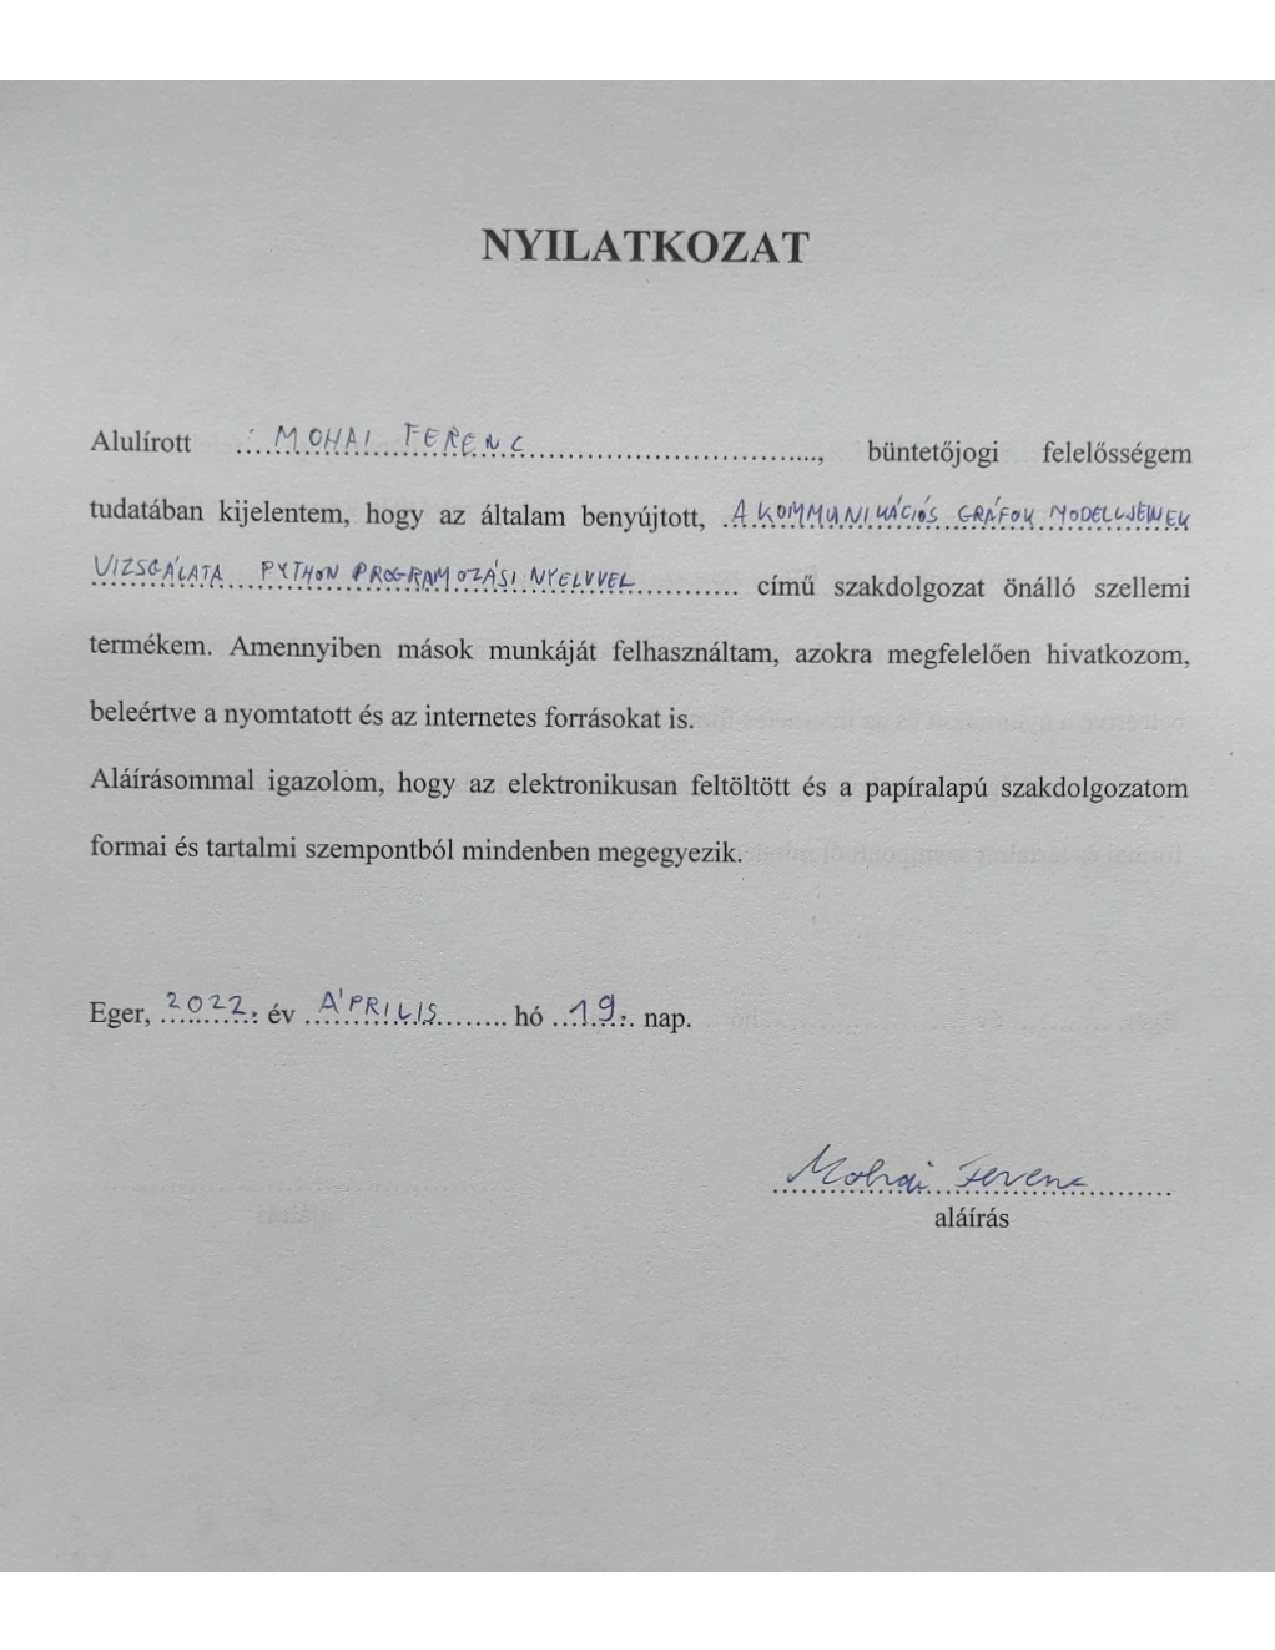
\includepdf[pagecommand={\thispagestyle{empty}}]{nyilatkozat.pdf}
\end{document}